% ------------------------------------------------------------------------------
% TYPO3 CMS 7.0 - What's New - Chapter "Deprecated Functions" (Spanish Version)
%
% @author	Michael Schams <schams.net>
% @author	Michel Mix <mmix@autistici.org>
% @license	Creative Commons BY-NC-SA 3.0
% @link		http://typo3.org/download/release-notes/whats-new/
% @language	Spanish
% ------------------------------------------------------------------------------
% LTXE-CHAPTER-UID:		daadb66f-be2ebc72-01347fcd-e99be5da
% LTXE-CHAPTER-NAME:	Deprecated Functions
% ------------------------------------------------------------------------------

\section{Funciones removidas/desvalorizadas}
\begin{frame}[fragile]
	\frametitle{Funciones removidas/desvalorizadas}

	\begin{center}\huge{Capítulo 5:}\end{center}
	\begin{center}\huge{\color{typo3darkgrey}\textbf{Funciones removidas/desvalorizadas}}\end{center}

\end{frame}

% ------------------------------------------------------------------------------
% LTXE-SLIDE-START
% LTXE-SLIDE-UID:		83a7d0b7-17e8280d-33aa4cc1-114755dd
% LTXE-SLIDE-ORIGIN:	c47248f9-03aa1da2-8dd9985d-762cf405 English
% LTXE-SLIDE-TITLE:		Legacy Layer
% LTXE-SLIDE-REFERENCE:	http://typo3.org/news/article/retaining-compatibility-to-typo3-cms6/
% ------------------------------------------------------------------------------

\begin{frame}[fragile]
	\frametitle{Funciones removidas/desvalorizadas}
	\framesubtitle{Capa de compatibilidad}

	\begin{itemize}

		\item TYPO3 CMS 6.2: una capa de compatibilidad se asegura que las extensiones antiguas funcionen en la nueva base de código\newline
			\small
				Desventaja: rendimiento disminuido (no el potencial completo del sistema)
			\normalsize

		\item TYPO3 CMS 7.0: capa de compatibilidad ha sido removida del núcleo\newline
			\small
				Impacto: las extensiones antiguas pueden fallar (por ejemplo, extensiones sin espacios de nombres)
			\normalsize

		\item La compatibilidad puede ser reforzada instalando extensión de sistema \texttt{EXT:compatibility6} si es requerido
		\item Esta extensión será movida a TER en el futuro

	\end{itemize}

\end{frame}

% ------------------------------------------------------------------------------
% LTXE-SLIDE-START
% LTXE-SLIDE-UID:		bd76c2db-81c50103-bd47e751-79fe1b5c
% LTXE-SLIDE-ORIGIN:	70da8aab-cd42e15f-fe254b81-41ceabb5 English
% LTXE-SLIDE-TITLE:		Backend User Management
% ------------------------------------------------------------------------------

\begin{frame}[fragile]
	\frametitle{Funciones removidas/desvalorizadas}
	\framesubtitle{Gestión de usuario de Backend}

	\begin{itemize}
		\item Ha sido removido el cambio a usuario de backend ("cambio-a-modo")
	\end{itemize}

	\smaller\tabto{1cm}\begingroup\color{typo3red}TYPO3 CMS 6.2\endgroup\normalsize
	\begin{figure}\vspace{-0.4cm}
		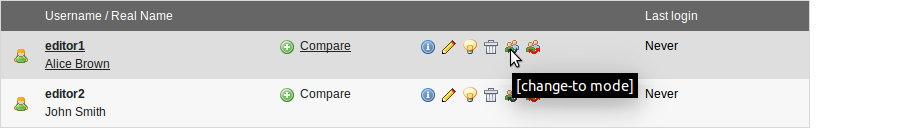
\includegraphics[width=0.90\linewidth]{DeprecatedRemovedFunctions/BackendUserSwitch1.png}
	\end{figure}

	\smaller\tabto{1cm}\begingroup\color{typo3red}TYPO3 CMS 7.0\endgroup\normalsize
	\begin{figure}\vspace{-0.4cm}
		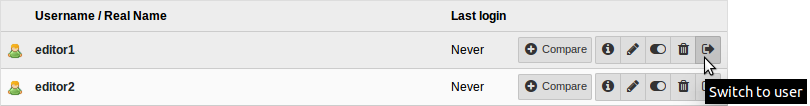
\includegraphics[width=0.90\linewidth]{DeprecatedRemovedFunctions/BackendUserSwitch2.png}
	\end{figure}

\end{frame}

% ------------------------------------------------------------------------------
% LTXE-SLIDE-START
% LTXE-SLIDE-UID:		6f0373d8-5428cfa6-8bfd63ce-11913719
% LTXE-SLIDE-ORIGIN:	10805d4d-787ce2f8-10e4329a-1451521a English
% LTXE-SLIDE-TITLE:		Removed Deprecated JavaScript Functions
% LTXE-SLIDE-REFERENCE:	https://github.com/TYPO3/TYPO3.CMS/commit/2dff81b963e1b77c7f068f91ffde73914a18b0be
% LTXE-SLIDE-REFERENCE:	https://forge.typo3.org/issues/62291
% LTXE-SLIDE-REFERENCE:	https://forge.typo3.org/projects/typo3cms-core/repository/revisions/9ac03e383e4786e868f4b1d81893e84c4621abc8/entry/typo3/sysext/core/Documentation/Changelog/master/Breaking-62291-RTEDeprecatedJavaScriptMethodsRemoved.rst
% ------------------------------------------------------------------------------

\begin{frame}[fragile]
	\frametitle{Funciones removidas/desvalorizadas}
	\framesubtitle{Funciones JavaScript removidas/desvalorizadas}

	\begin{itemize}
		\item De acuerdo con la \href{http://forge.typo3.org/projects/typo3v4-core/wiki/CoreDevPolicy}{estrategia de desvalorización},
			algunos métodos de JavaScript clasificados como \textit{desvalorizados} desde TYPO3 CMS 4.7, han sido removidos, por ejemplo:

		\begin{lstlisting}
			\TYPO3\CMS\Backend\Form\FormEngine->getSingleField_typeInput
			\TYPO3\CMS\Backend\Form\FormEngine->getSingleField_typeText
			\TYPO3\CMS\Core\Utility\GeneralUtility->quoted_printable
			\TYPO3\CMS\Core\Utility\GeneralUtility->encodeHeader
		\end{lstlisting}

		\smaller
			\texttt{HTMLArea.Editor.forceRedraw}\newline
				(use \texttt{HTMLArea.Framework.doLayout} en su lugar)
				\vspace{0.2cm}

			\texttt{HTMLArea.Editor.convertNode}\newline
				(use \texttt{HTMLArea.DOM.convertNode} en su lugar)
				\vspace{0.2cm}

			\texttt{HTMLArea.Editor.getBlockAncestors}\newline
				(use \texttt{HTMLArea.DOM.getBlockAncestors} en su lugar)
		\normalsize

	\end{itemize}

\end{frame}

% ------------------------------------------------------------------------------
% LTXE-SLIDE-START
% LTXE-SLIDE-UID:		9d40d668-eb809cd4-a8eae0c7-5fe7a666
% LTXE-SLIDE-ORIGIN:	9da41efc-970e66a8-f9163c40-67cfa712 English
% LTXE-SLIDE-TITLE:		Removed Functions (1)
% LTXE-SLIDE-REFERENCE:	https://forge.typo3.org/issues/17579
% LTXE-SLIDE-REFERENCE:	https://forge.typo3.org/issues/62888
% ------------------------------------------------------------------------------

\begin{frame}[fragile]
	\frametitle{Funciones removidas/desvalorizadas}
	\framesubtitle{Funciones removidas}

	\begin{itemize}

		\item
			\small
				TypoScript setting \texttt{config.uniqueLinkVars} ha sido removido\newline
				(este comportamiento está por defecto ahora)
			\normalsize

		\item
			\small
				ViewHelper
					\texttt{\textbackslash
						TYPO3\textbackslash
						CMS\textbackslash
						Documentation\textbackslash
						ViewHelpers\textbackslash
						Link\textbackslash
						Action}
					ha sido removido (use \texttt{f:be.buttons.icon} o \texttt{f:uri.*} en su lugar)
			\normalsize

		\item
			\small
				Opción PageTSconfig \texttt{mod.web\_list.alternateBgColors}\newline
				ha sido removido
			\normalsize

		\item
			\small
				PropertyMapper ha sido removido\newline
				(including option \texttt{rewrittenPropertyMapper = 0})
			\normalsize

		\item
			\small
				Las condiciones TypoScript han sido removidas:

					\begin{itemize}
						\item\texttt{browser}
						\item\texttt{version}
						\item\texttt{system}
						\item\texttt{useragent}
					\end{itemize}
			\normalsize

	\end{itemize}

\end{frame}

% ------------------------------------------------------------------------------
% LTXE-SLIDE-START
% LTXE-SLIDE-UID:		ccab1ce8-878e5ecb-470d78dc-6a5900d3
% LTXE-SLIDE-ORIGIN:	efe86631-b6020ae8-ffa01160-6de29dc3 English
% LTXE-SLIDE-TITLE:		Removed Functions (1)
% ------------------------------------------------------------------------------

\begin{frame}[fragile]
	\frametitle{Funciones removidas/desvalorizadas}
	\framesubtitle{Métodos removidos (1)}

	Los siguientes \textbf{métodos} han sido removidos:

	\begin{itemize}
		\item
			\small
				\texttt{connectDB}\newline
				de la clase
				\texttt{\textbackslash
					TYPO3\textbackslash
					CMS\textbackslash
					Frontend\textbackslash
					Utility\textbackslash
					EidUtility}
			\normalsize
		\item
			\small
				\texttt{isDisplayCondition}\newline
				de la clase
				\texttt{\textbackslash
					TYPO3\textbackslash
					CMS\textbackslash
					Form\textbackslash
					FormEngine}
			\normalsize
		\item
			\small
				\texttt{int\_from\_ver}\newline
				de la clase
				\texttt{\textbackslash
					TYPO3\textbackslash
					CMS\textbackslash
					Core\textbackslash
					Utility\textbackslash
					GeneralUtility}
			\normalsize
		\item
			\small
				\texttt{getUniqueFields}\newline
				de la clase
				\texttt{\textbackslash
					TYPO3\textbackslash
					CMS\textbackslash
					Core\textbackslash
					DataHandling\textbackslash
					DataHandler}
			\normalsize

	\end{itemize}

\end{frame}

% ------------------------------------------------------------------------------
% LTXE-SLIDE-START
% LTXE-SLIDE-UID:		0d22c9db-a82901f5-93030e98-3a14ac8d
% LTXE-SLIDE-ORIGIN:	293414d4-e87db3d5-afced471-ca9826ed English
% LTXE-SLIDE-TITLE:		Removed Methods (2)
% ------------------------------------------------------------------------------

\begin{frame}[fragile]
	\frametitle{Funciones removidas/desvalorizadas}
	\framesubtitle{Métodos removidos (2)}

	Los siguientes \textbf{métodos} han sido removidos:

	\begin{itemize}

		\item
			\small
				\texttt{isSafeModeEnabled}\newline
				de la clase
				\texttt{\textbackslash
					TYPO3\textbackslash
					CMS\textbackslash
					Core\textbackslash
					Utility\textbackslash
					PhpOptionsUtility}
			\normalsize
		\item
			\small
				\texttt{registerSwiftMailer}\newline
				de la clase
				\texttt{\textbackslash
					TYPO3\textbackslash
					CMS\textbackslash
					Core\textbackslash
					Bootstrap}
			\normalsize
		\item
			\small
				\texttt{loadTCA}\newline
				de la clase
				\texttt{\textbackslash
					TYPO3\textbackslash
					CMS\textbackslash
					Core\textbackslash
					Utility\textbackslash
					GeneralUtility}
			\normalsize
		\item
			\small
				\texttt{isLocalconfWritable}\newline
				de la clase
				\texttt{\textbackslash
					TYPO3\textbackslash
					CMS\textbackslash
					Core\textbackslash
					Utility\textbackslash
					ExtensionManagementUtility}
			\normalsize

	\end{itemize}

\end{frame}

% ------------------------------------------------------------------------------
% LTXE-SLIDE-START
% LTXE-SLIDE-UID:		7bb49218-4a3c3f30-bbdafdc1-ba68d535
% LTXE-SLIDE-ORIGIN:	a1ba1998-f88c1063-71470741-30b9f314 English
% LTXE-SLIDE-TITLE:		Removed Classes
% ------------------------------------------------------------------------------

\begin{frame}[fragile]
	\frametitle{Funciones removidas/desvalorizadas}
	\framesubtitle{Clases removidas}

	Las siguientes \textbf{clases} han sido removidas:

	\begin{itemize}

		\item
			\smaller
				\texttt{\textbackslash
					TYPO3\textbackslash
					CMS\textbackslash
					Backend\textbackslash
					Template\textbackslash
					MediumDocumentTemplate}
			\normalsize
		\item
			\smaller
				\texttt{\textbackslash
					TYPO3\textbackslash
					CMS\textbackslash
					Extbase\textbackslash
					Service\textbackslash
					TypeHandlingService}
			\normalsize

	\end{itemize}

\end{frame}

% ------------------------------------------------------------------------------
